\documentclass[9pt,aspectratio=169,t]{beamer}
\usepackage[T1]{fontenc}
\usepackage{lmodern,amsmath,amssymb,mathtools,booktabs,array,graphicx}
\usefonttheme{professionalfonts}
\hypersetup{pdftitle={Structural Crowding Allocation},pdfauthor={Jamshid Ardalankia},pdfsubject={Correlation-profile diversification under systemic stress}}
\definecolor{blueink}{HTML}{184F86}
\definecolor{ink}{HTML}{202B34}
\definecolor{subtle}{HTML}{4B5C68}
\definecolor{hairline}{HTML}{CBD6DD}
\setbeamercolor{normal text}{fg=ink,bg=white}
\setbeamercolor{structure}{fg=blueink}
\setbeamersize{text margin left=7.2mm,text margin right=7.0mm}
\setbeamerfont{normal text}{size=\fontsize{8.0}{10.2}}
\setbeamertemplate{navigation symbols}{}
\setbeamertemplate{background canvas}{\color{blueink}\rule{1.08mm}{\paperheight}}
\setbeamerfont{frametitle}{family=\rmfamily,series=\bfseries,size=\fontsize{14.2}{16.2}}
\setbeamercolor{frametitle}{fg=ink}
\newcommand{\sectiontag}{Motivation}
\setbeamertemplate{frametitle}{\nointerlineskip\vspace*{3.3mm}%
 {\color{blueink}\sffamily\bfseries\fontsize{6.0}{7.1}\selectfont\MakeUppercase{\sectiontag}\par}%
 \vspace{1.15mm}{\usebeamerfont{frametitle}\color{ink}\insertframetitle\par}\vspace{1.25mm}%
 {\color{hairline}\hrule height .38pt}\vspace{1.25mm}}
\newcommand{\scaFooterTextFont}{\fontsize{5.5}{6.3}\selectfont}
\newcommand{\scaFooterPageFont}{\fontsize{6.4}{7}\selectfont}
\setbeamertemplate{footline}{\leavevmode\hbox to\paperwidth{\hskip7.2mm{\color{subtle}\scaFooterTextFont \insertauthor\hspace{1.25mm}/\hspace{1.25mm}Structural Crowding Allocation}\hfil{\color{blueink}\scaFooterPageFont \insertframenumber}\hskip7.0mm}\vskip2.1mm}
\newcommand{\src}[1]{\par\vfill\vspace{.7mm}{\raggedright\color{subtle}\fontsize{5.7}{7.0}\selectfont #1\par}}
\newcommand{\lab}[1]{{\color{blueink}\sffamily\bfseries #1}}
\newcommand{\headrow}[1]{\par\noindent\lab{#1}\par\vspace{.6mm}}
\newcommand{\halfline}{\par\vspace{1.1mm}{\color{hairline}\hrule height .35pt}\vspace{1.2mm}}
\newcommand{\smath}{\fontsize{7.8}{9.65}\selectfont\setlength{\abovedisplayskip}{1.8pt}\setlength{\belowdisplayskip}{1.8pt}\setlength{\abovedisplayshortskip}{1pt}\setlength{\belowdisplayshortskip}{1.6pt}\setlength{\jot}{1.8pt}}
\newcommand{\norm}[1]{\left\lVert #1\right\rVert}
\newcommand{\W}{\mathcal W}
\newcommand{\one}{\mathbf 1}
\newcommand{\tv}{\mathrm{TV}}
\newcommand{\algn}[1]{\mathrm{align}_{#1}^{P,\tv}}
\newcommand{\SL}{\mathrm{SL}}
\newcommand{\ML}{\mathrm{ML}}
\newcommand{\HY}{\mathrm{HY}}
\newcommand{\MV}{\mathrm{MV}}
\newcommand{\raw}{\mathrm{raw}}
\DeclareMathOperator{\tr}{tr}
\DeclareMathOperator{\diag}{diag}
\DeclareMathOperator*{\argmin}{arg\,min}
\title{Structural Crowding Allocation}
\author{Jamshid Ardalankia}
\begin{document}

% Slide 01 - Structural Crowding Allocation
\begin{frame}[plain]
\vspace*{17.5mm}
{\rmfamily\bfseries\color{ink}\fontsize{20.8}{24}\selectfont Structural Crowding Allocation\par}
\vspace{2.5mm}
{\rmfamily\color{subtle}\fontsize{12.3}{15.1}\selectfont Price and Trading Value Correlation-Profile Diversification\\under Systemic Stress\par}
\vspace{5mm}{\color{blueink}\rule{12mm}{.8pt}}\par\vspace{4mm}
{\bfseries\fontsize{7.85}{10.25}\selectfont Jamshid Ardalankia}\par\vspace{.8mm}
{\color{subtle}\fontsize{6.45}{8.45}\selectfont Department of Economics, Virginia Tech, USA}

\par\vspace{.8mm}
{\color{subtle}\fontsize{6.45}{8.45}\selectfont Southern Economic Association Annual Meeting, Houston TX, 2026}
\end{frame}

% Opening frames share a smaller footer.
\begingroup
\renewcommand{\scaFooterTextFont}{\fontsize{4.75}{5.5}\selectfont}
\renewcommand{\scaFooterPageFont}{\fontsize{5.5}{6.45}\selectfont}
% Slide 02 - Same direct correlation, different neighbors
\begin{frame}{Same direct correlation, different neighbors}
\setlength{\unitlength}{1mm}
\noindent\begin{picture}(145,13)(0,-7)
  % The line enters from the page edge and ends at the open research question.
  \color{blueink}\linethickness{1.25pt}
  \put(-7.2,0){\line(1,0){142}}
  \put(18,0){\circle*{1.8}}
  \put(61,0){\circle*{1.8}}
  \put(106,0){\circle*{1.8}}
  \put(18,2.5){\makebox(0,0)[b]{\fontsize{8.0}{9.0}\selectfont\bfseries
    \href{https://doi.org/10.1007/s100510050929}{Mantegna (1999)}}}
  \put(61,2.5){\makebox(0,0)[b]{\fontsize{8.0}{9.0}\selectfont\bfseries
    \href{https://doi.org/10.1140/epjb/e2002-00380-9}{Onnela et al.\ (2002)}}}
  \put(106,2.5){\makebox(0,0)[b]{\fontsize{8.0}{9.0}\selectfont\bfseries
    \href{https://doi.org/10.1016/j.jempfin.2016.06.003}{Peralta \& Zareei (2016)}}}
  \put(140,0){\makebox(0,0){\rmfamily\bfseries\fontsize{16}{16}\selectfont ?}}
  \color{subtle}\fontsize{5.85}{7.7}\selectfont
  \put(18,-2.3){\makebox(0,0)[t]{Stock-return correlation trees}}
  \put(61,-2.3){\makebox(0,0)[t]{Markowitz portfolios on the tree}}
  \put(106,-2.3){\makebox(0,0)[t]{Portfolio selection by centrality}}
\end{picture}\par
\vspace{.5mm}
\begin{columns}[c,onlytextwidth]
\begin{column}{.43\textwidth}
  \centering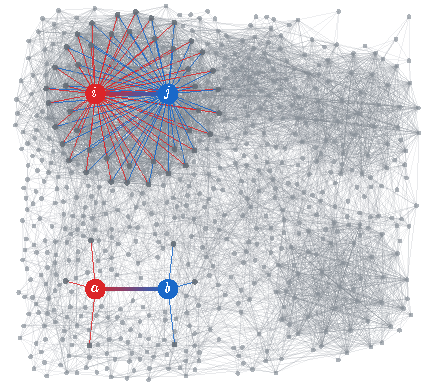
\includegraphics[width=\linewidth,height=35.5mm,keepaspectratio]{network.pdf}
\end{column}
\begin{column}{.55\textwidth}
  {\fontsize{7.4}{9.95}\selectfont
    Both pairs have the same direct correlation, $\rho^P_{ij}=\rho^P_{ab}$.
    The upper pair shares more neighbors.\par}
  \vspace{2.6mm}
  {\color{blueink}\bfseries\fontsize{9.4}{11.1}\selectfont Structural Crowding Allocation (SCA)\par}
  \vspace{1.0mm}
  {\fontsize{7.4}{9.95}\selectfont
    A portfolio is structurally crowded when much of its weight is in stocks with similar correlation profiles.
    SCA accounts for this overlap alongside covariance risk when setting weights.\par}
\end{column}
\end{columns}
\vfill
{\color{hairline}\hrule height .45pt}\vspace{1.4mm}
{\color{blueink}\rmfamily\bfseries\fontsize{8.75}{11.25}\selectfont
Can using correlation-profile similarity as an additional diversification criterion reduce portfolio drawdowns during systemic stress?\par}
\note{Pause at the question mark, then point to the two highlighted pairs.
These two pairs have the same direct correlation. What if one pair shares many more neighbors?}
\end{frame}

\renewcommand{\sectiontag}{This paper}
% Slide 03 - An additional diversification criterion
\begin{frame}{An additional diversification criterion}
\vspace*{-2.0mm}
{\fontsize{7.55}{9.6}\selectfont I use overlap in stocks' correlation profiles alongside covariance risk when setting portfolio weights.\par}
\vspace{1.1mm}
\begingroup
\fontsize{8.7}{10.25}\selectfont
\setlength{\tabcolsep}{0pt}
\renewcommand{\arraystretch}{.94}
\begin{tabular}{@{}l@{\hspace{1.8mm}}r@{\hspace{.55mm}}c@{\hspace{.55mm}}c@{\hspace{.75mm}}c@{\hspace{.75mm}}r@{\hspace{1mm}}l@{}}
{\lab{\fontsize{8.25}{9.2}\selectfont Portfolio variance}}&
\(w^\top\Sigma w\)&\(=\)&
\(\sum\nolimits_i w_i^2\Sigma_{ii}\)&\(+\)&
\(2\sum\nolimits_{i<j} w_i w_j\,{\color{blueink}\Sigma_{ij}}\)&\\[.5mm]
{\lab{\fontsize{8.25}{9.2}\selectfont Structural crowding}}&
\(C(w)=w^\top S w\)&\(=\)&
\(\underbrace{\displaystyle\sum_{i=1}^{N} w_i^{2}S_{ii}}_{\text{\sffamily\color{subtle}\fontsize{5.9}{7.05}\selectfont individual profile terms}}\)&\(+\)&
\(\underbrace{\displaystyle 2\sum_{1\le i<j\le N} w_iw_j\,{\color{blueink}S_{ij}}}_{\text{\sffamily\color{subtle}\fontsize{5.9}{7.05}\selectfont joint profile interactions}}\)&
\(=\displaystyle\left\lVert\sum_i w_i\boldsymbol{\phi}_i\right\rVert_2^{\,2}\)
\end{tabular}\par
\endgroup
\vspace{.65mm}
{\color{subtle}\fontsize{6.8}{8.45}\selectfont
For fitted stock profiles \(\boldsymbol{\phi}_i\), \(S_{ij}=\langle\boldsymbol{\phi}_i,\boldsymbol{\phi}_j\rangle\) and \(\sum_i w_i\boldsymbol{\phi}_i\) is the portfolio profile.\par}
\vspace{1.0mm}{\color{hairline}\hrule height .42pt}\vspace{2.55mm}

\begin{columns}[T,onlytextwidth]
\begin{column}{.455\textwidth}
{\lab{\fontsize{9.6}{10.8}\selectfont Single-Layer (SL)}\par}
\vspace{.55mm}
{\fontsize{7.15}{9}\selectfont
Keep the positive part of stock \(i\)'s return correlation with each of the \(N\) stocks.\par}
\vspace{.8mm}
{\fontsize{7.85}{9.85}\selectfont
\(z_i^P=\bigl([\rho^P_{ik}]_+\bigr)_{k=1}^{N},\qquad
[x]_+=\max(x,0)\).\par}
\vspace{1.0mm}
{\fontsize{8.15}{10.25}\selectfont
\(S_{ij}^{\SL,\raw}=\dfrac{\langle z_i^P,z_j^P\rangle}{N}
=\dfrac{1}{N}\displaystyle\sum_{k=1}^{N}[\rho_{ik}^P]_+[\rho_{jk}^P]_+\).\par}
\end{column}
\begin{column}{.507\textwidth}
{\lab{\fontsize{9.6}{10.8}\selectfont Multilayer (ML)}\hfill
{\color{subtle}\fontsize{6.2}{7.7}\selectfont \href{https://doi.org/10.1371/journal.pone.0330372}{Building on Ardalankia et al.\ (2025)}}\par}
\vspace{.55mm}
{\fontsize{7.15}{9}\selectfont Form \(z_i^{\tv}\) from daily log changes in trading value (TV).\par}
\vspace{.55mm}
{\fontsize{7.85}{9.65}\selectfont
\begin{tabular}{@{}l@{\hspace{2mm}}l@{}}
\(K_{ij}^{\tv}=\tfrac{1}{N}\langle z_i^{\tv},z_j^{\tv}\rangle\)
 & {\fontsize{6.7}{8.45}\selectfont TV overlap of \(i\) and \(j\)}\\[.75mm]
\(\varphi_i^{P,\tv}=\tfrac{1}{N}\langle z_i^P,z_i^{\tv}\rangle\)
 & {\fontsize{6.7}{8.45}\selectfont Stock \(i\) across layers}\\[.75mm]
\(\displaystyle S_{ij}^{\ML,\raw}=\varphi_i^{P,\tv}K_{ij}^{\tv}\varphi_j^{P,\tv}\)
 & {\fontsize{6.7}{8.45}\selectfont ML similarity of \(i\) and \(j\)}
\end{tabular}\par}
\end{column}
\end{columns}
\vspace{1.0mm}{\color{hairline}\hrule height .42pt}\vspace{.75mm}
\noindent
{\lab{\fontsize{9.6}{10.8}\selectfont Hybrid (HY)}}\hspace{2.8mm}
{\fontsize{8.7}{10.7}\selectfont
\(\widetilde S^{\HY}=\tfrac12\widetilde S^{\SL}+\tfrac12\widetilde S^{\ML}\)}\hspace{2.8mm}
{\fontsize{7.05}{9}\selectfont The baseline averages the two trace-normalized matrices.}
\note{Start with portfolio variance. What if two holdings move with the same other stocks? SCA adds their profile overlap as a diversification criterion. Point to the two underbraces and the squared norm. Explain stock-pair overlap on the source layer before same-stock alignment across layers. The bilateral portfolio construction builds on the interlayer similarity in Ardalankia et al. (2025). In the main specification the Hybrid gives equal weight to the separately fitted and trace-normalized matrices. Once I have the structural matrix, how should it affect portfolio weights?}
\end{frame}

\renewcommand{\sectiontag}{Allocation rules}
% Slide 04 - Three ways to allocate using the same structural matrix
\begin{frame}{Three ways to allocate using the same structural matrix}
\vspace*{-5.15mm}

% Shared notation, aligned across the slide.
\noindent
\begin{minipage}[t]{.345\textwidth}\raggedright
  {\color{subtle}\fontsize{8.1}{9.5}\selectfont Risk with trace-normalized covariance\par}
  \vspace{1.05mm}
  {\fontsize{7.6}{9.8}\selectfont \(V(w)=w^\top\widetilde\Sigma w\)\par}
\end{minipage}\hfill
\begin{minipage}[t]{.295\textwidth}\raggedright
  {\color{subtle}\fontsize{8.1}{9.5}\selectfont Profile crowding (SL, ML or HY)\par}
  \vspace{1.05mm}
  {\fontsize{7.6}{9.8}\selectfont \(C(w)=w^\top S w\)\par}
\end{minipage}\hfill
\begin{minipage}[t]{.31\textwidth}\raggedright
  {\color{subtle}\fontsize{8.1}{9.5}\selectfont Long-only, fully invested\par}
  \vspace{1.05mm}
  {\fontsize{7.6}{9.8}\selectfont
   \(w\in\mathcal W=\{w\geq0,\ \mathbf1^\top w=1\}\)\par}
\end{minipage}\par
\vspace{3.14mm}{\color{hairline}\hrule height .42pt}

% Method descriptions and equations occupy separate, vertically centered columns.
\nointerlineskip\begin{minipage}[t][17.7mm][c]{\textwidth}
\noindent\begin{minipage}[c]{.29\textwidth}\raggedright
  {\lab{\fontsize{10.6}{12.2}\selectfont Composite SCA}\par}
  \vspace{.8mm}
  {\fontsize{7.3}{9.45}\selectfont Minimize the weighted sum of variance and crowding.\par}
\end{minipage}\hfill
\begin{minipage}[c]{.63\textwidth}\raggedright
  {\fontsize{7.8}{10.0}\selectfont
   \(Q_\alpha=(1-\alpha)\widetilde\Sigma+\alpha S,\qquad
     {\color{blueink}\alpha=0.50}\ \text{(baseline)}.\)\par}
  \vspace{2.7mm}
  {\fontsize{7.8}{10.0}\selectfont
   \(w^{\rm comp}=\displaystyle\argmin_{w\in\mathcal W} w^\top Q_\alpha w.\)\par}
\end{minipage}
\end{minipage}\par
\nointerlineskip{\color{hairline}\hrule height .36pt}

\nointerlineskip\begin{minipage}[t][15.8mm][c]{\textwidth}
\noindent\begin{minipage}[c]{.29\textwidth}\raggedright
  {\lab{\fontsize{10.6}{12.2}\selectfont Risk-Parity SCA}\par}
  \vspace{.8mm}
  {\fontsize{7.3}{9.45}\selectfont Equalize each stock's share of composite risk.\par}
\end{minipage}\hfill
\begin{minipage}[c]{.63\textwidth}\raggedright
  {\fontsize{8.05}{10.4}\selectfont
   \(\displaystyle r_i^Q(w)=\frac{w_i(Q_\alpha w)_i}{w^\top Q_\alpha w}
      ={\color{blueink}\frac1N},\qquad w_i>0,\quad i=1,\ldots,N.\)\par}
\end{minipage}
\end{minipage}\par
\nointerlineskip{\color{hairline}\hrule height .36pt}

\nointerlineskip\begin{minipage}[t][22.6mm][c]{\textwidth}
\noindent\begin{minipage}[c]{.29\textwidth}\raggedright
  {\lab{\fontsize{10.6}{12.2}\selectfont Constrained SCA}\par}
  \vspace{.8mm}
  {\fontsize{7.3}{9.45}\selectfont Minimize crowding within a cap on estimated volatility.\par}
  \vspace{1.65mm}
  {\color{subtle}\fontsize{6.65}{8.65}\selectfont
   10\% min. \(\xrightarrow{\kappa=2\%}\) {\bfseries\color{blueink}10.2\%} cap.\par}
\end{minipage}\hfill
\begin{minipage}[c]{.63\textwidth}\raggedright
  {\fontsize{7.8}{10.0}\selectfont
   \(C_\eta(w)=w^\top S_\eta w
       =\sum\nolimits_i w_i^2 S_{ii}
        +2{\color{blueink}\eta}\sum\nolimits_{i<j}w_iw_j S_{ij}.\)\par}
  \vspace{2.8mm}
  {\fontsize{7.8}{10.0}\selectfont
   \(w^{\rm C}\in\displaystyle\argmin_{w\in\mathcal W} C_\eta(w)
       \quad\text{subject to}\quad V(w)\leq(1+{\color{blueink}\kappa})^2v_{\MV}.\)\par}
  \vspace{1.7mm}
  {\color{subtle}\fontsize{7.2}{9.25}\selectfont
   \(v_{\MV}=\min_{u\in\mathcal W} V(u)\).\par}
\end{minipage}
\end{minipage}\par
\note{Hold the structural matrix fixed. Composite SCA minimizes a weighted sum of covariance risk and structural crowding. Risk-Parity SCA uses the same composite matrix and equalizes every stock's relative contribution. Constrained SCA puts an explicit limit on estimated volatility and then minimizes structural crowding within that limit. The 10 percent illustration concerns an estimate at portfolio formation.}
\end{frame}
\endgroup

\renewcommand{\sectiontag}{Empirical design}
% Slide 05 - Data, rolling windows and benchmarks
\begin{frame}{Data, rolling windows and benchmarks}
\smath
\begin{columns}[T,onlytextwidth]
\begin{column}{.50\textwidth}
\headrow{Investment universe}
At each formation date, select 100 liquid companies from historical S\&P 500 membership, ranked by trailing median Trading Value. All strategies use the same eligible stocks.
\vspace{2.2mm}
\headrow{Estimation and investment}
Estimate from 504 trading days of CRSP data through $t$. Choose weights at $t$ and evaluate simple returns over the following 63 trading days. Weights drift between rebalances.
\vspace{2.2mm}
\headrow{Out-of-sample period}
95 formations and 5,985 investment days, 8 January 2002 to 20 October 2025. GFC and COVID are evaluation periods.
\end{column}
\begin{column}{.456\textwidth}
\headrow{Conventional allocation}
Equal Weight and three minimum-variance portfolios: sample, Ledoit--Wolf (LW) and analytical nonlinear shrinkage (NLS).
\vspace{2.2mm}
\headrow{Network portfolios}
HRP allocates recursively through a hierarchy. PZ Lowest-Centrality and PZ Rho-Dependent each select 20 stocks.
\vspace{2.2mm}
\headrow{Contribution budgeting}
Covariance ERC gives each stock an equal contribution to covariance risk. It is the matched budgeting benchmark for Risk-Parity SCA.
\end{column}
\end{columns}
\src{Article, Section 4 and Tables 1--2. The estimation inputs are log returns and log changes in Trading Value. CAGR and volatility are annualized; drawdown is the peak-to-trough loss within the evaluation window.}
\end{frame}

\renewcommand{\sectiontag}{Empirical evidence}
% Seven results frames for the main conference talk.
% Slide 06 - Profile overlap near minimum variance
\begin{frame}{Profile overlap near minimum variance}
At each formation, Constrained SCA may take up to \textbf{2\% more estimated volatility} than its matching minimum-variance portfolio.

\vspace{0.65em}
\begin{center}
\small
\renewcommand{\arraystretch}{1.32}
\begin{tabular}{@{}lrl@{}}
\toprule
Profile architecture & Mean reduction in full-matrix exposure & \\
\midrule
Single-Layer & 34.68\% & \textcolor{blueink}{\rule{2.50cm}{.72ex}} \\
Multilayer   & 38.63\% & \textcolor{blueink}{\rule{2.79cm}{.72ex}} \\
Hybrid       & 33.03\% & \textcolor{blueink}{\rule{2.38cm}{.72ex}} \\
\bottomrule
\end{tabular}
\end{center}
\vspace{0.35em}
\small At formation $t$, both portfolios use the same architecture-specific $S_t$ for evaluation:
\[
  \text{reduction}_{t}=100\!\left[1-
  \frac{(w_{t}^{C})^{\mathsf T}S_t w_{t}^{C}}
       {(w_{t}^{\mathrm{MV}})^{\mathsf T}S_t w_{t}^{\mathrm{MV}}}\right].
\]
The table averages these reductions. Optimization uses $S_{\eta,t}$ with $\eta=0.50$.
\src{Section 5.1, p. 13. Average across 95 formation dates.}
\end{frame}

% Slide 07 - Risk parity changes portfolio breadth and turnover
\begin{frame}{Risk parity changes portfolio breadth and turnover}
\small Full sample. Composite ML and Risk-Parity ML use the same matrix $Q_{0.50}$.

\begin{center}
\small
\renewcommand{\arraystretch}{1.25}
\begin{tabular}{@{}lrr@{}}
\toprule
Allocation & Effective holdings & Annual one-way turnover \\
\midrule
Composite ML      & 13.8 & 99.2\% \\
Risk-Parity ML    & \textbf{87.0} & \textbf{37.5\%} \\
Covariance ERC    & 85.5 & 31.9\% \\
\bottomrule
\end{tabular}
\end{center}

\small Equalizing contributions spreads capital across more stocks and reduces trading relative to minimizing the same criterion. Covariance ERC achieves similar breadth with lower turnover.
\src{Table 10, p. 26. Effective holdings $=1/\sum_i w_i^2$ at target weights. Descriptive full-sample comparisons.}
\end{frame}

% Slide 08 - GFC performance across the three allocation rules
\begin{frame}{GFC performance across the three allocation rules}
\begin{columns}[T,onlytextwidth]
\begin{column}{.59\textwidth}
\small Gross returns, July 2007--June 2009
\vspace{0.24em}

\footnotesize
\setlength{\tabcolsep}{4.1pt}
\renewcommand{\arraystretch}{1.04}
\begin{tabular}{@{}lrrr@{}}
\toprule
Allocation & CAGR & Vol. & MaxDD \\
\midrule
Composite SL       & $-10.83$ & 27.59 & 44.77 \\
Constrained ML     & $-9.61$  & 23.98 & 34.63 \\
Risk-Parity ML     & $-21.41$ & 37.42 & 58.03 \\
\midrule
LW MinVar          & $-8.41$  & 23.49 & 34.44 \\
NLS MinVar         & $-8.82$  & 23.61 & 34.81 \\
HRP                & $-16.05$ & 30.87 & 49.22 \\
Covariance ERC     & $-19.37$ & 35.56 & 54.96 \\
PZ Lowest          & $-24.14$ & 31.92 & 60.14 \\
PZ Rho-Dependent   & $-25.88$ & 34.19 & 62.30 \\
\bottomrule
\end{tabular}
\end{column}
\begin{column}{.39\textwidth}
\small
\textbf{Composite SL} gained 13.30 and 15.05 percentage points in CAGR versus PZ Lowest and PZ Rho-Dependent, respectively. Four loss measures also improved against each. All ten comparisons meet Holm-adjusted 5\% within the stated families.

\medskip
\textbf{Constrained ML} had drawdown close to both MinVar benchmarks.

\medskip
\textbf{Risk-Parity ML} had deeper drawdown than Covariance ERC.
\end{column}
\end{columns}
\src{Tables 3B and 6. All entries in percent. ML uses $h=1$. Composite/Risk-Parity: $\alpha=0.50$. Constrained: $\kappa=2\%$, $\eta=1$.}
\end{frame}

% Slide 09 - COVID crash losses and recovery participation
\begin{frame}{COVID crash losses and recovery participation}
\begin{columns}[T,onlytextwidth]
\begin{column}{.52\textwidth}
\small Gross cumulative return (\%) by phase
\vspace{0.24em}

\footnotesize
\setlength{\tabcolsep}{5pt}
\renewcommand{\arraystretch}{1.13}
\begin{tabular}{@{}lrr@{}}
\toprule
Allocation & Crash & Recovery \\
\midrule
Composite ML    & $-35.15$ & 68.31 \\
Constrained ML  & $-35.06$ & 56.71 \\
Risk-Parity ML  & $-33.17$ & 87.17 \\
Risk-Parity HY  & $-32.71$ & 84.21 \\
\midrule
LW MinVar       & $-36.00$ & 48.82 \\
Covariance ERC  & $-32.88$ & 82.91 \\
HRP             & $-31.75$ & 75.11 \\
Both PZ rules   & $-28.35$ & 77.90 \\
Equal Weight    & $-33.58$ & 92.32 \\
\bottomrule
\end{tabular}
\end{column}
\begin{column}{.46\textwidth}
\small
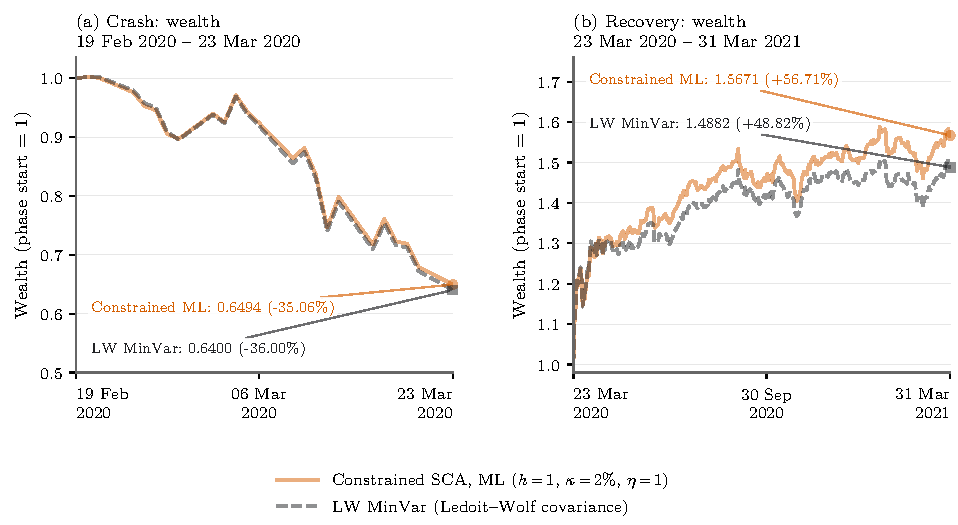
\includegraphics[width=\linewidth]{covid.pdf}\par
{\scriptsize Constrained ML and LW MinVar. Wealth restarts at one in each phase.}\par
\medskip
Risk-Parity ML and HY exceeded Covariance ERC in recovery. Equal Weight gained the most.
\end{column}
\end{columns}
\src{Figure 4 and Tables 7, 9A. Crash: 20 Feb--23 Mar 2020. Recovery: 24 Mar 2020--31 Mar 2021. Descriptive returns. Constrained: $\kappa=2\%$, $\eta=1$.}
\end{frame}

% Slide 10 - Sensitivity to the volatility allowance
\begin{frame}{Sensitivity to the volatility allowance}
\small Constrained ML with $h=1$ and $\eta=0.50$. Only $\kappa$ changes.

\begin{center}
\small
\renewcommand{\arraystretch}{1.22}
\begin{tabular}{@{}lrr@{}}
\toprule
Measure & $\kappa=2\%$ & $\kappa=5\%$ \\
\midrule
Mean reduction in full-matrix exposure & 38.63\% & 53.65\% \\
Effective holdings at formation & 13.56 & 15.14 \\
\midrule
GFC maximum drawdown & 34.34\% & 35.65\% \\
COVID and recovery CAGR & 4.91\% & 9.21\% \\
\bottomrule
\end{tabular}
\end{center}

\small The wider allowance buys more profile diversification. It coincides with a deeper GFC drawdown and higher compound growth over the COVID-and-recovery window.
\src{Section 5.5 and Figure 6, p. 22. Financial outcomes are descriptive.}
\end{frame}

% Slide 11 - What does trading value add?
\begin{frame}{What does trading value add?}
\small Constrained SCA with the same universe, covariance estimate, $2\%$ allowance and full interaction weight ($\eta=1$). Only the structural architecture changes.

\begin{center}
\small
\renewcommand{\arraystretch}{1.20}
\setlength{\tabcolsep}{5pt}
\begin{tabular}{@{}lrrrrr@{}}
\toprule
& \multicolumn{3}{c}{Portfolio outcome} & \multicolumn{2}{c}{Holm-adjusted $p$} \\
\cmidrule(lr){2-4}\cmidrule(l){5-6}
Full-sample measure (\%) & SL & ML & HY & ML vs. SL & HY vs. SL \\
\midrule
Annualized volatility           & 14.886 & 14.586 & 14.752 & 0.0003 & 0.0029 \\
Annualized downside deviation   & 10.563 & 10.343 & 10.472 & 0.0018 & 0.0229 \\
Daily ES95                      &  2.197 &  2.142 &  2.178 & 0.0033 & 0.0275 \\
\midrule
Maximum drawdown                & 37.25 & 35.58 & 36.41 & 0.7863 & 0.7863 \\
\bottomrule
\end{tabular}
\end{center}

\small ML and HY lower volatility, downside deviation and expected shortfall relative to SL. The drawdown, CAGR and Sharpe differences fall short of adjusted 5\%.
\src{Table 8A, p. 24. Holm adjustment across architecture pairs within each metric. $h=1$, hybrid weight $\gamma=0.50$.}
\end{frame}

% Slide 12 - Full-sample growth and loss control
\begin{frame}{Full-sample growth and loss control}
\begin{columns}[T,onlytextwidth]
\begin{column}{.59\textwidth}
\small Gross returns, January 2002--October 2025
\vspace{0.24em}

\footnotesize
\setlength{\tabcolsep}{4.1pt}
\renewcommand{\arraystretch}{1.03}
\begin{tabular}{@{}lrrr@{}}
\toprule
Allocation & CAGR & Vol. & MaxDD \\
\midrule
Composite SL     &  7.72 & 16.59 & 44.77 \\
Constrained ML   &  7.74 & 14.59 & 35.58 \\
Risk-Parity ML   &  9.19 & 19.83 & 58.03 \\
\midrule
LW MinVar        &  7.09 & 14.42 & 36.46 \\
NLS MinVar       &  7.15 & 14.35 & 35.17 \\
HRP              &  9.04 & 17.04 & 49.22 \\
Covariance ERC   &  9.07 & 18.86 & 54.96 \\
PZ Lowest        & 10.37 & 18.14 & 60.14 \\
PZ Rho-Dependent & 10.93 & 19.66 & 62.30 \\
Equal Weight     &  8.92 & 21.62 & 60.40 \\
\bottomrule
\end{tabular}
\end{column}
\begin{column}{.39\textwidth}
\small
\textbf{Growth.} Both PZ rules have higher compound growth than the three SCA portfolios shown.

\medskip
\textbf{Loss control.} Constrained ML remains close to shrinkage MinVar on volatility and drawdown.

\medskip
\textbf{Risk budgeting.} Covariance ERC has lower volatility and drawdown than Risk-Parity ML.
\end{column}
\end{columns}
\src{Table 3A, p. 14. Descriptive percentages. The three SCA specifications match the GFC comparison.}
\end{frame}

\renewcommand{\sectiontag}{Conclusion}
% Slide 13 - What does structural crowding add?
\begin{frame}{What does structural crowding add?}
\vspace{1.3mm}
{\rmfamily\fontsize{10.7}{13.5}\selectfont A portfolio can spread capital across names while repeatedly holding the same dependence profile. $C(w)$ makes that overlap an explicit allocation choice.\par}
\vspace{3mm}
\headrow{A risk allowance makes the trade-off measurable}
Across the three architectures, a 2\% estimated-volatility allowance reduced full-matrix profile exposure by 33--39\% relative to matching MinVar.
\vspace{2.2mm}
\headrow{Loss control depends on the benchmark}
In the GFC, Composite SL improved growth and four loss measures relative to both PZ rules. Constrained ML had drawdown close to LW and NLS MinVar.
\vspace{2.2mm}
\headrow{A risk budget changes the investment outcome}
Risk-Parity ML held more effective assets and traded less than Composite ML. It gained more than covariance ERC in the COVID recovery, with higher volatility over the full sample.
\src{Sections 5.1--5.8; Tables 3, 6, 7 and 10.\hfill\texttt{ardalankia@vt.edu}}
\end{frame}

\renewcommand{\sectiontag}{Technical appendix}
% Slide 14 - Structural marginal costs and risk contributions
\begin{frame}{Structural marginal costs and risk contributions}
\smath
\begin{columns}[T,onlytextwidth]
\begin{column}{.474\textwidth}
\headrow{What does another dollar add?}
For a fitted symmetric $S$, the marginal structural cost of asset $i$ depends on the current portfolio:
\[
 \frac{\partial C(w)}{\partial w_i}=2(Sw)_i=2\sum_j S_{ij}w_j.
\]
When $\Delta$ of portfolio weight moves from $j$ to $i$,
\[
 \begin{aligned}
 C(w+\Delta(e_i-e_j))-C(w)
 &=2\Delta\{(Sw)_i-(Sw)_j\}\\
 &\quad+\Delta^2(S_{ii}+S_{jj}-2S_{ij}).
 \end{aligned}
\]
For Constrained SCA the diagonal contribution stays fixed as a function of $\eta$:
\[
 w^\top S_\eta w=\sum_i w_i^2 S_{ii}+2\eta\sum_{i<j}w_iw_jS_{ij}.
\]
\end{column}
\begin{column}{.49\textwidth}
\headrow{Which contributions does Risk-Parity equalize?}
Let $Q_\alpha=B_\alpha+E$, where $E$ collects numerical conditioning, and let $q=w^\top Q_\alpha w$. Write
\[
 \begin{aligned}
 r_i^{\Sigma}&=\frac{(1-\alpha)w_i(\widetilde\Sigma w)_i}{q},\qquad
 r_i^S=\frac{\alpha w_i(Sw)_i}{q},\\[1mm]
 r_i^{E}&=\frac{w_i(Ew)_i}{q},\qquad
 r_i^Q=r_i^\Sigma+r_i^S+r_i^E=\frac{1}{N}.
 \end{aligned}
\]
The equal budget applies to the sum. Individual covariance and structural contributions can differ across stocks.
\vspace{2mm}
\headrow{Two checks}
At $\alpha=0$ the budgets apply to covariance alone; at $\kappa=0$ the constrained feasible set contains only the matching minimum-variance optimum.
\end{column}
\end{columns}
\src{Equations (3.3)--(3.5), (3.10)--(3.12), (3.19)--(3.21); Online Appendix S5, S9 and S26.}
\end{frame}

\end{document}
